\newpage
\section{Auswertung}
\label{sec:Auswertung}

% Subfigure ein bisschen klein, leider
%\begin{figure}
%    \begin{subfigure}{0.5\textwidth}
%        \centering
%        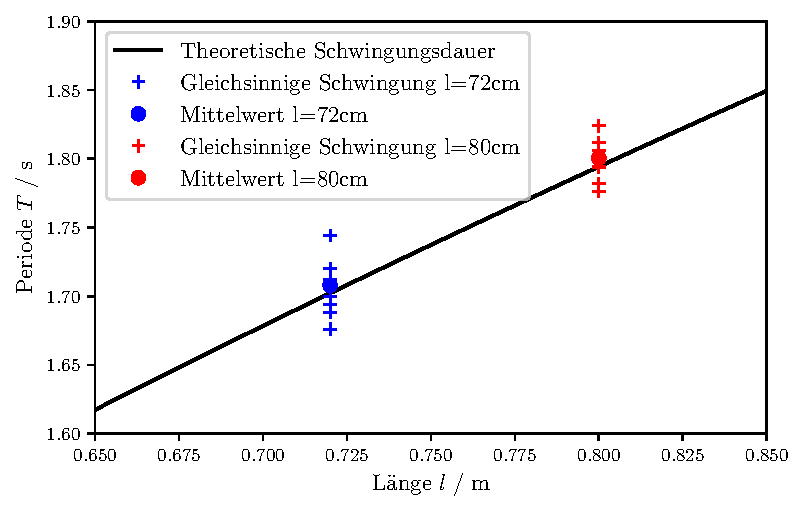
\includegraphics[width=\textwidth]{build/plot1.pdf}
%        \caption{$f(x)=|sin(x)|$}
%    \end{subfigure}
%    \begin{subfigure}{0.5\textwidth}
%        \centering
%        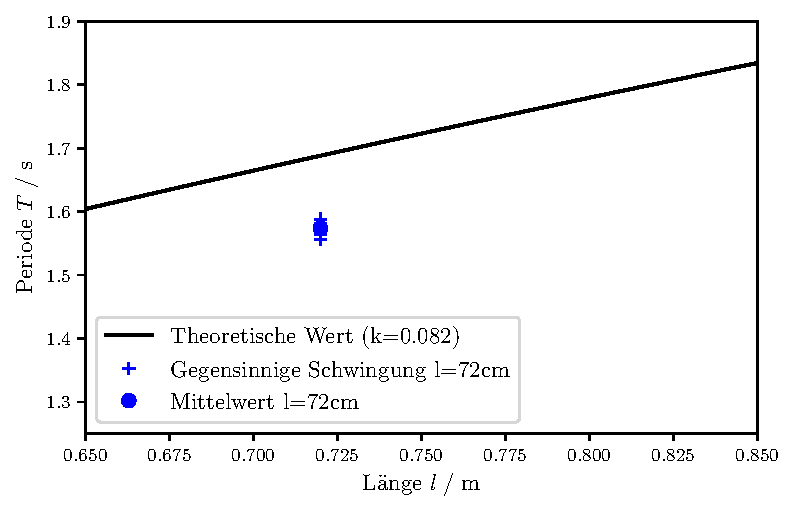
\includegraphics[width=\textwidth]{build/plot2.pdf}
%        \caption{$f(x)=x$}
%    \end{subfigure}
%    \caption{Fouriersynthese}
%\end{figure}

Nach den Integrationen, ergeben sich folgende Werte für die verschiedenen $\omega_k$ für die Koeffizenten $A_k$ und $B_k$

\begin{table}
\centering
    \begin{tabular}{S[table-format=3.1] S S S S}
        \toprule
        & \multicolumn{2}{c}{$f_2(x)=x$} & \multicolumn{2}{c}{$f_1(x)=|sin(x)|$} \\
        \cmidrule(lr){2-3}\cmidrule(lr){4-5}
        {$k$} & {$A_k$} & {$B_k$} & {$A_k$} & {$B_k$}\\
        \midrule
         0 & 0 &  0.00 &  0.636619 & 0 \\
         1 & 0 &  2.00 & -0.424413 & 0 \\
         2 & 0 & -0.99 & -0.084883 & 0 \\
         3 & 0 &  0.66 & -0.036378 & 0 \\
         4 & 0 & -0.49 & -0.020210 & 0 \\
         5 & 0 &  0.39 & -0.012861 & 0 \\
         6 & 0 & -0.33 & -0.008904 & 0 \\
         7 & 0 &  0.28 & -0.006529 & 0 \\
         8 & 0 & -0.24 & -0.004993 & 0 \\
         9 & 0 &  0.22 & -0.003942 & 0 \\
        10 & 0 & -0.20 & -0.003191 & 0 \\
        11 & 0 &  0.18 & -0.002636 & 0 \\
        12 & 0 & -0.16 & -0.002214 & 0 \\
        13 & 0 &  0.15 & -0.001886 & 0 \\
        14 & 0 & -0.14 & -0.001626 & 0 \\
        15 & 0 &  0.13 & -0.001416 & 0 \\
        16 & 0 & -0.12 & -0.001245 & 0 \\
        17 & 0 &  0.12 & -0.001102 & 0 \\
        \bottomrule
    \end{tabular}
    \caption{Koeffizenten $A_k$ und $B_k$}
    \label{tab:tabelle}
\end{table}
\newpage

Mit dem Programm Fouriersynthese \cite{Fouriersynthese} lassen sich mit den Koeffizenten \ref{tab:tabelle} die Fouriersynthesen darstellen.

\begin{figure}
    \centering
    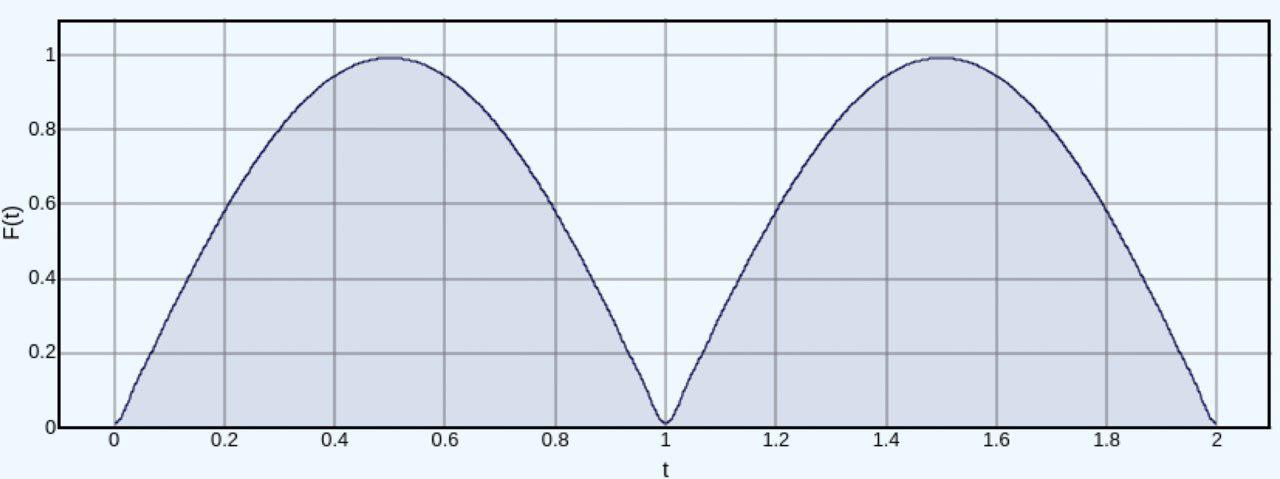
\includegraphics[width=\textwidth]{website/sin.jpg}
    \caption{Fouriersynthese für $f(x)=|sin(x)|$}
\end{figure}


\begin{figure}
    \centering
    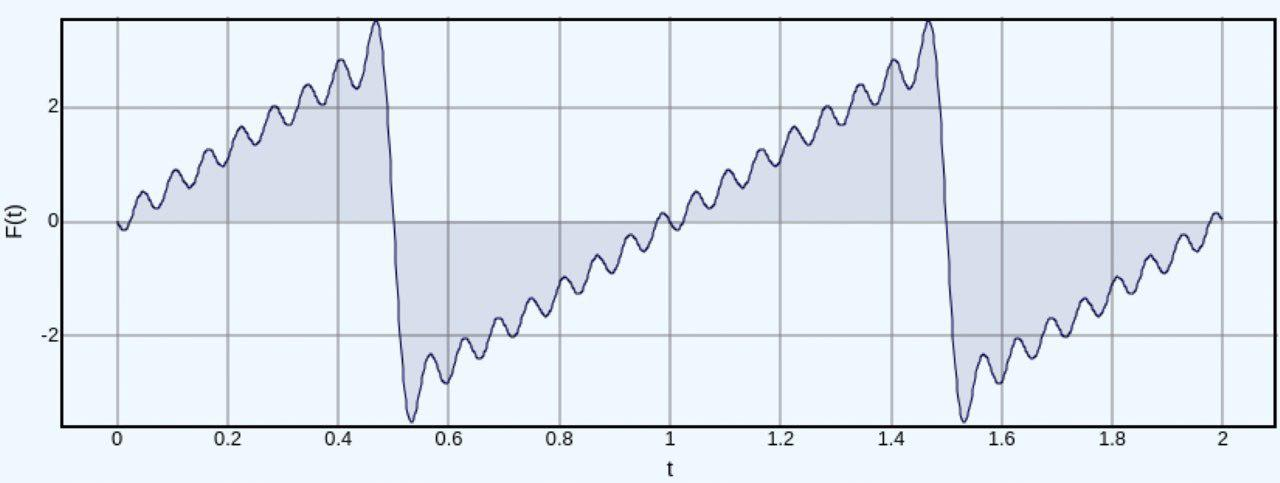
\includegraphics[width=\textwidth]{website/x.jpg}
    \caption{Fouriersynthese für $f(x)=x$}
    \label{fig:x_website}
\end{figure}
Die Skalierung der x-Achse, ist bei dieser Abbildung \ref{fig:x_website} irreführend, da das Programm \cite{Fouriersynthese} keine Möglichkeit gibt eine Periode $T$ anzugeben 
und somit $T=2\pi$ vorraussetzt.

\newpage

Die Exaktheit der Synthese, wir beim Übereinanderlegen mit der originalen Funktion deutlich.
\begin{figure}
    \centering
    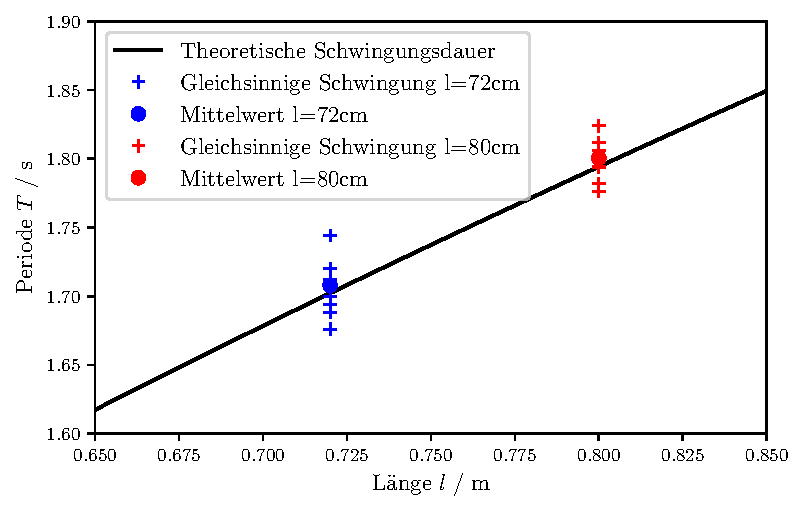
\includegraphics[width=0.75\textwidth, height=0.4635\textwidth]{build/plot1.pdf}
    \caption{Fouriersynthese für $f_1(x)=|sin(x)|$}
    \label{fig:FS_sin}
\end{figure}

\begin{figure}
    \centering
    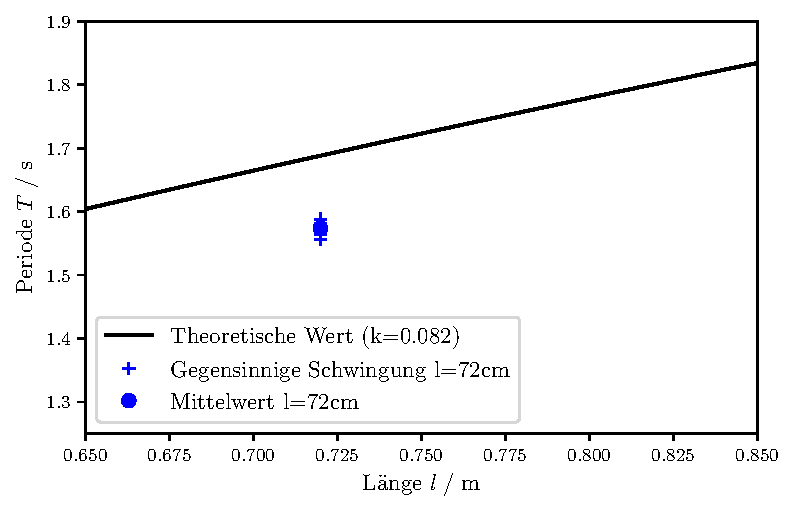
\includegraphics[width=0.75\textwidth, height=0.4635\textwidth]{build/plot2.pdf}
    \caption{Fouriersynthese für $f_2(x)=x$}
    \label{fig:FS_x}
\end{figure}
